\section*{Task 1}
NOT gates with BJT transistors (NPN)

a)RTL
\begin{figure}[H] 
\begin{center}
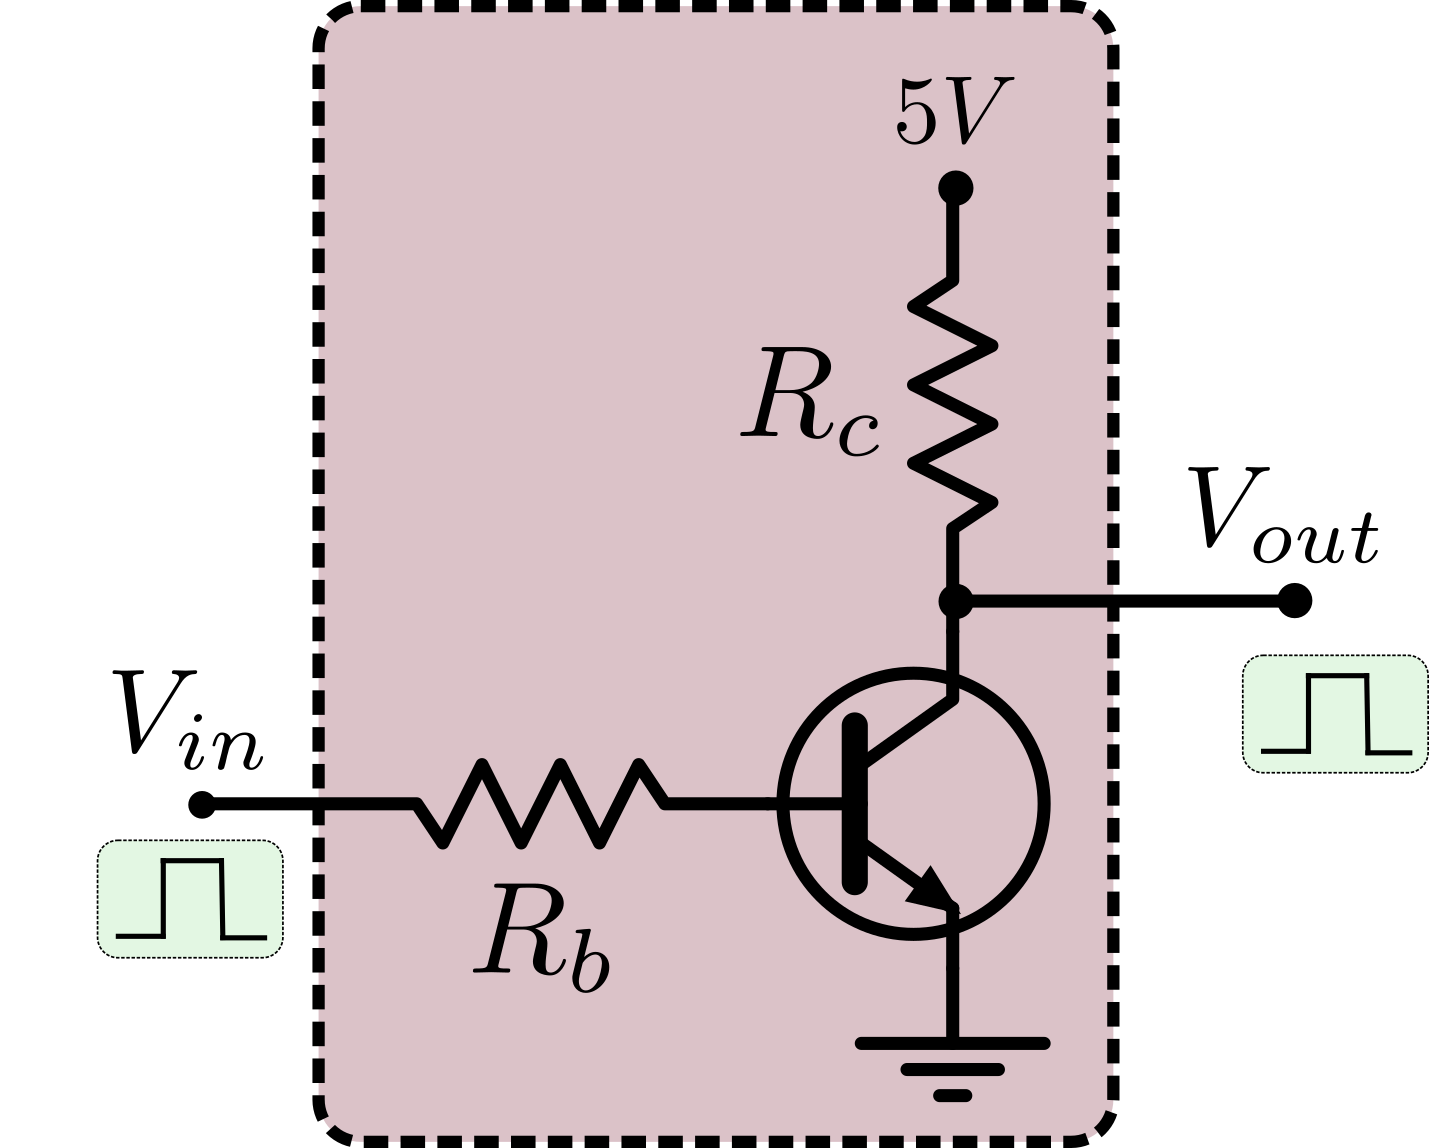
\includegraphics[width=8.25cm,height=8cm]{data/1a.png}
\end{center}
\caption{}
\label{fig:ej1a}
\end{figure} 

b) TTL

\begin{figure}[H] 
\begin{center}
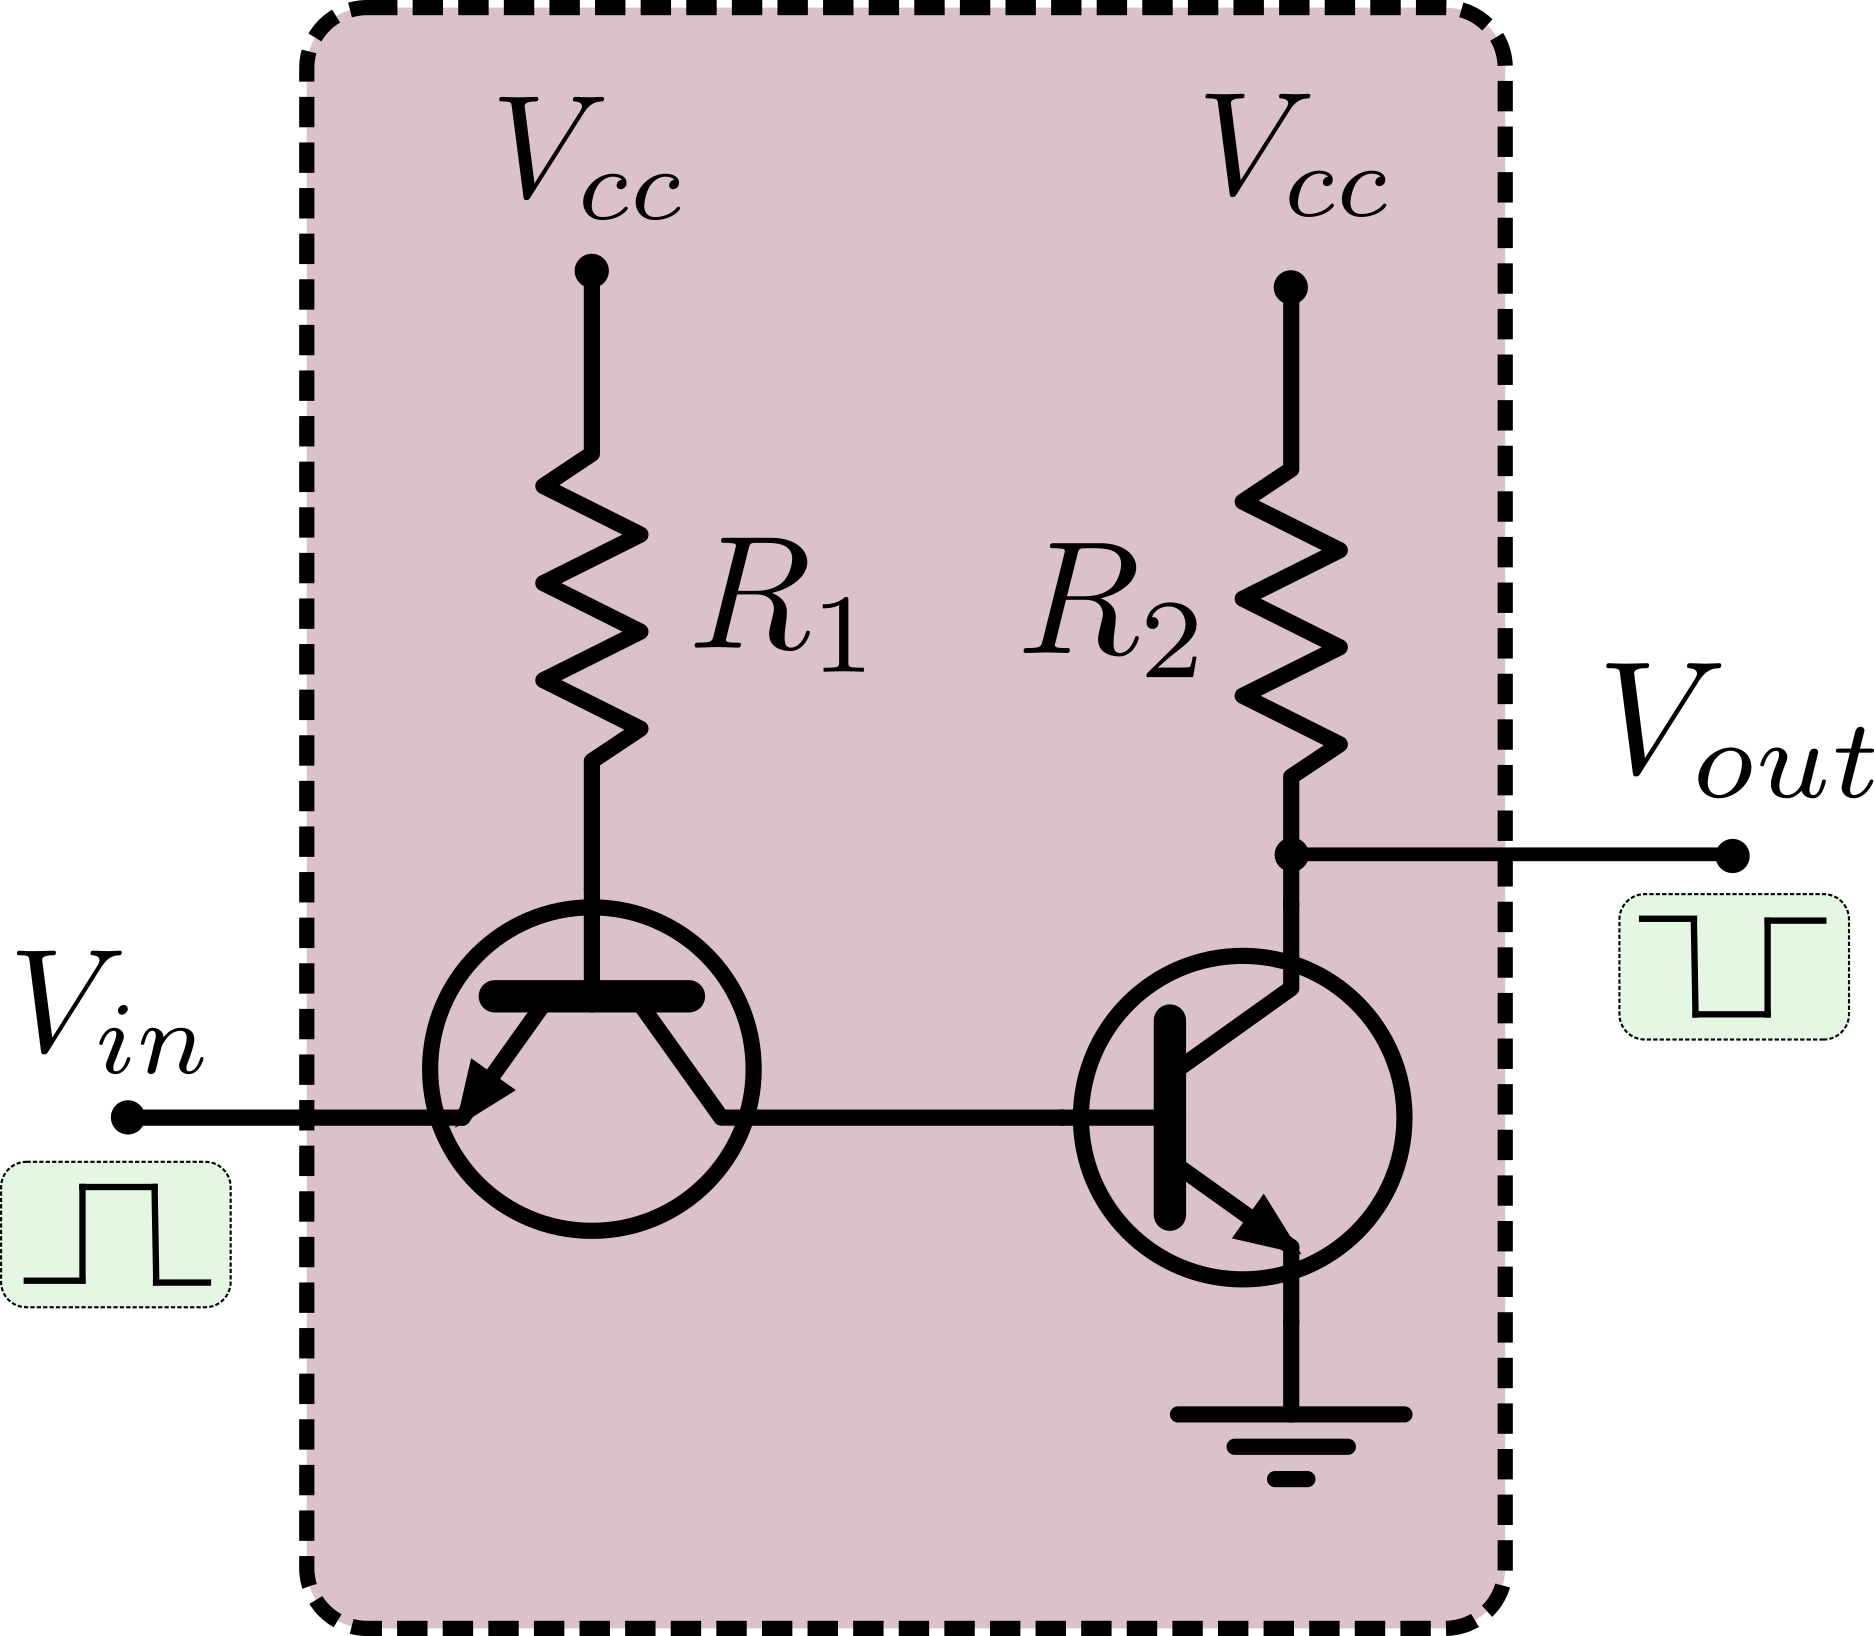
\includegraphics[width=8.25cm,height=8cm]{data/1b.png}
\end{center}
\caption{}
\label{fig:ej1b}
\end{figure} 

\section*{MEASSURES}
\begin{figure}[H] 
\begin{center}
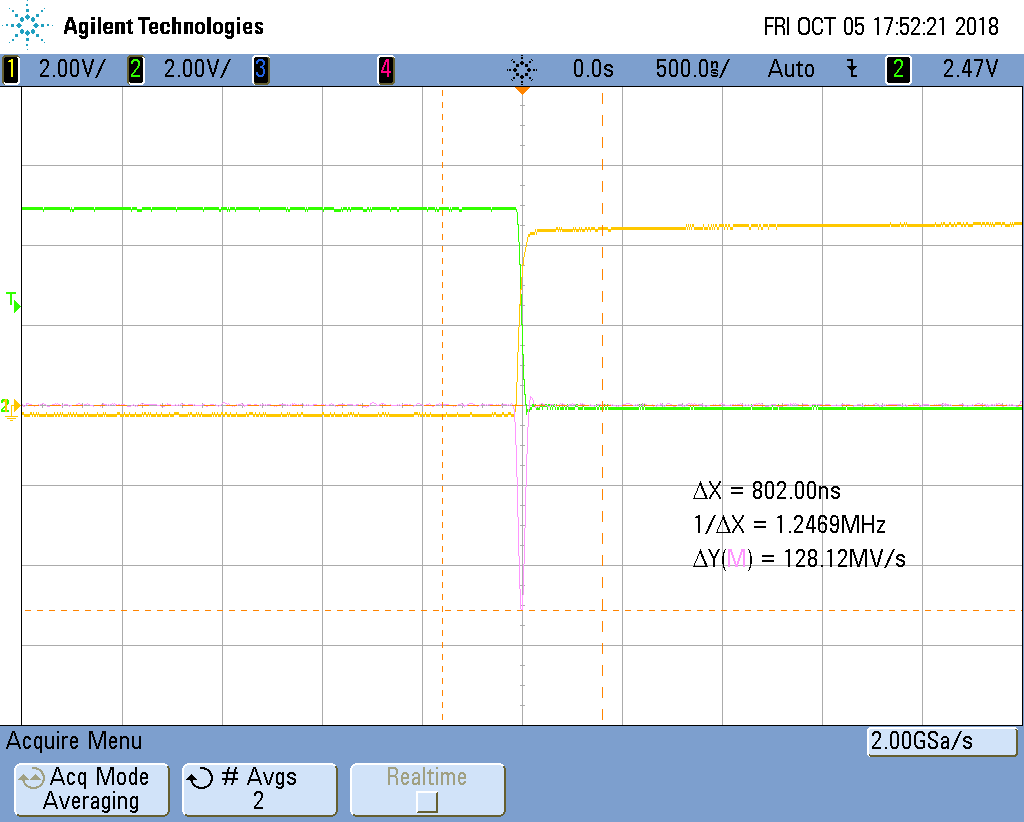
\includegraphics[width=8.25cm,height=8cm]{data/imax1.png}
\end{center}
\caption{}
\label{fig:measures}
\end{figure} 

Where $V_{IH}$: minimum HIGH input voltage, $V_{IL}$: maximum LOW input voltage, $V_{OH}$: minimum HIGH output voltage, $V_{OL}$: maximum LOW output voltage.

To meassure these values we use the ramp waveform and the oscilloscope in xy mode so we can see something like this:
\begin{figure}[H] 
    \begin{center}
    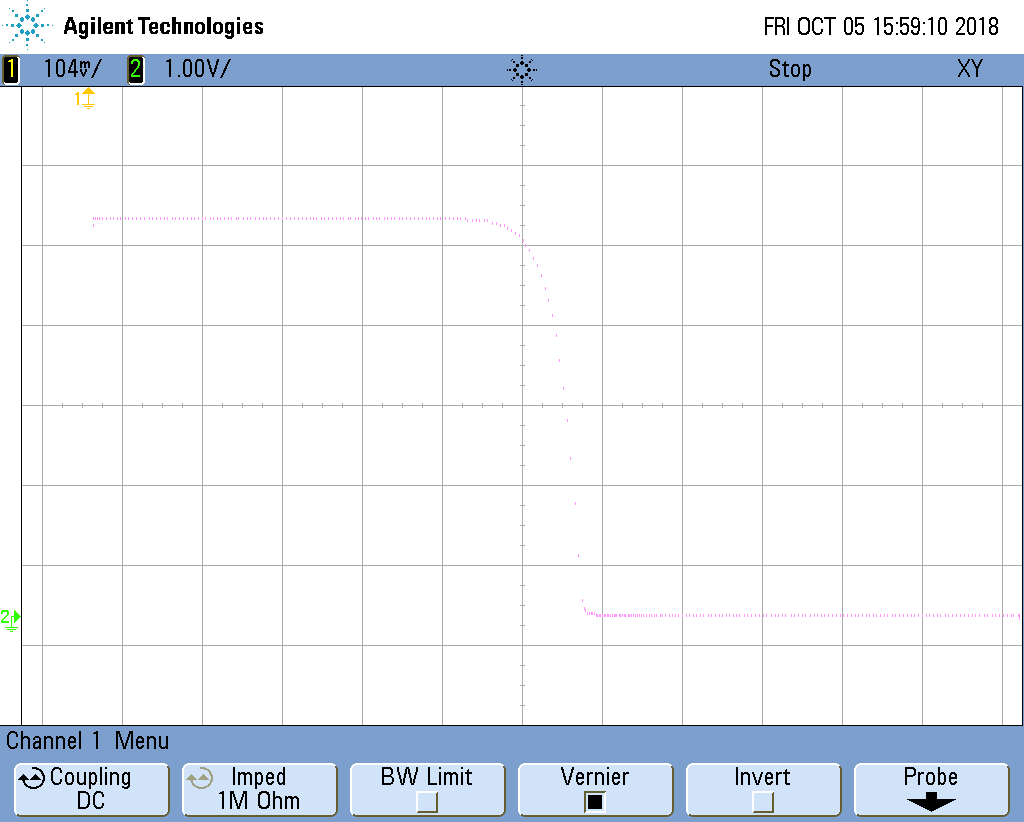
\includegraphics[width=8.25cm,height=8cm]{data/xy_ttl_bjt.png}
    \end{center}
    \caption{}
    \label{fig:measures}
    \end{figure}     
Where the values we are looking for are found when the derivative is -1.

Noise margin :It allows one to estimate the allowable noise voltage on the input of a 
gate so that the output will not be affected. Noise margin is specified
 in terms of two parameters: the low noise margin $N_{L}$, and the high noise 
 margin $N_{H}$ . $N_{L}$ is defined as the difference in magnitude
  between the maximum LOW input voltage and the maximum 
  LOW output voltage of the gate. That is, $N_{L}$ =$|V_{IL} - V_{OL}|$.
   Similarly, the value of $N_{H}$ is the difference in 
   magnitude between the minimum HIGH output voltage of 
   and the minimum HIGH input voltage recognizable by 
   the gate. That is, $N_{H} =|V_{OH} - V_{IH}|.$ 


The propagation delay  is the difference in time (calculated at 50
\% of input-output transition), when output switches, after 
application of input. It is different if the transition is
 from HIGH to LOW or form LOW to HIGH.

 Rise time is the time, during transition, when output switches from 10\% to 90\% of the maximum value.
Fall time is the time when output switches from 90\% to 10\% of the maximum value.

In order to get the maximum output current, knowing that the
 load is a 1nF capacitor, with the oscilloscope we find out
  the derivative of the output voltage:
\begin{equation}
    i_{c}=C\frac{dV_{OUT}}{dt}
\end{equation}
The maximum current is when the derivative is maximum.
\subsection*{a)1)no load}
$V_{OL}$=244mV ;
$V_{OH}$=4,85V ; 
$V_{IL}$=547mV ;
$V_{IH}$=1,83V
\newline
Rise time = 1,26 us 
\newline
Fall time = 410 ns 
\newline 
Propagation time (HIGH to LOW) = 2,86 us 
\newline
Propagation time (LOW to HIGH) = 520 ns.
\newline
There is not a maximum output current because there is no load.

\subsection*{a)2)with load} 

$V_{OL}$=384mV ; 
$V_{OH}$=4,75V ; 
$V_{IL}$=584mV ;
$V_{IH}$=1,76V 
\newline
Rise time = 1,76 us
\newline
Fall time = 480 ns
\newline
Propagation time (HIGH to LOW) = 3,12 us
\newline
Propagation time (LOW to HIGH) = 656 ns
\newline
Max current when input goes from LOW to HIGH: -9,38 mA
\newline
Max current when input goes from HIGH to LOW: 2,66 mA
\subsection*{b)1)no load}
$V_{OL}$=100mV ; 
$V_{OH}$=4,69V ; 
$V_{IL}$=570mV ; 
$V_{IH}$=680mV 
\newline
Rise time = 156 ns
\newline
Fall time = 27 ns
\newline
Propagation time (HIGH to LOW) = 299 ns
\newline
Propagation time (LOW to HIGH) $<$ 13ns
\newline
It was not possible to determine because of the signal generator limitations
(the square wave rise/fall time is $<$13ns)
there is not a maximum output current because there is no load. 

\subsection*{b)2)with load} 

$V_{OL}$= 70mV ; 
$V_{OH}$= 4,68V ; 
$V_{IL}$= 550mV ;
$V_{IH}$= 700mV
\newline
Rise time = 960 ns
\newline
Fall time = 28 ns
\newline
Propagation time (HIGH to LOW) = 1,11 us
\newline
Propagation time (LOW to HIGH) $<$ 13 ns
\newline
Max current when input goes from LOW to HIGH: -128 mA
\newline
Max current when input goes from HIGH to LOW: 8,75 mA
\newline
There are 2 different currents because when the transistor
 is in saturation mode, the capacitor discharges on the 
 NPN transistor that has no resistance. And in cut off
  mode the capacitor charges with the resistance.

